\section{Compiler/System Optimization} 
\label{sec:system_optimization}

After model compression and algorithm optimization for LLMs, the next step is to compile and deploy them on hardware devices. To ensure efficient inference of LLMs, there are various compiler optimizations that can be employed.
Moreover, due to the increasing scale of LLMs, multiple hardware devices may be required for deployment and execution, forming a complex inference infrastructure system. As a result, system-level optimization for efficient inference has become a hot topic.
In this section, we will explore some widely used compiler optimization and system optimization techniques. 
These include operator fusion, memory management, workload offloading, and parallel serving.

% the next step is to compile the models and deployed on hardware devices.
% There are some compile optimization can be used for efficient inference of LLMs.
% Furthermore, because the scale of LLMs are increasing, they requires more than one hardware devices to deploy and execute, constituting a system of inference infrastructure.
% Therefore, the system-level optimization for efficiently inference has become a hot topic.
% In this section, we will survey some popular compile and system optimization techniques, including operator fusion, memory management, workload offloading and parallel serving.

\subsection{Operator Fusion}

\begin{figure}[t]
    \centering
    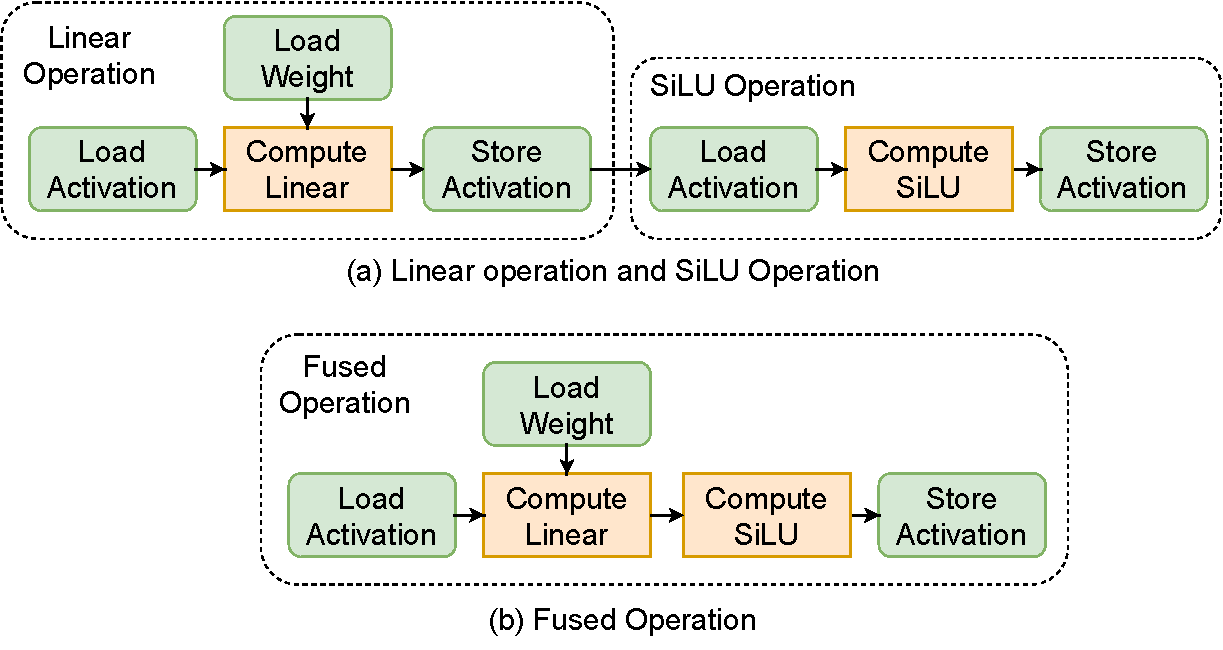
\includegraphics[width=0.95\linewidth]{ims/operator_fusion.pdf}
    % \vspace{-0.6in}
    \caption{Demonstration of operator fusion for a linear operator followed by a SiLU operator.}
    \label{fig:operator_fusion}
\end{figure}

\begin{figure}[t]
    \centering
    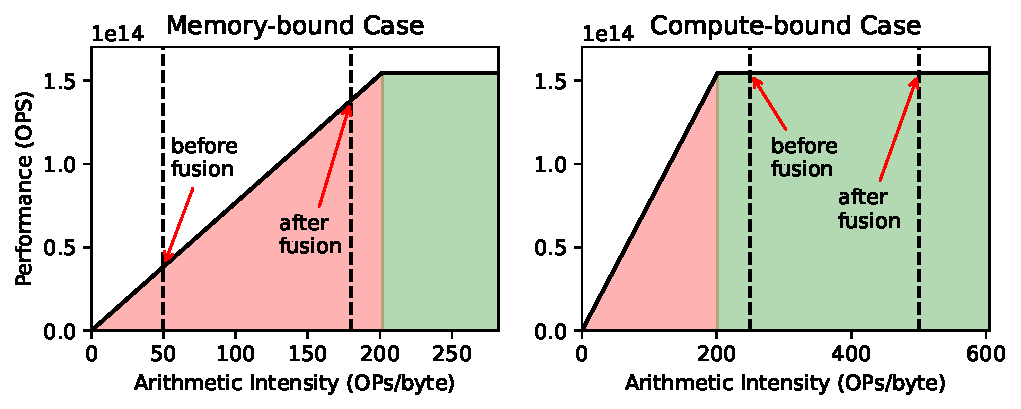
\includegraphics[width=0.95\linewidth]{ims/roofline_operator_fusion.pdf}
    % \vspace{-0.6in}
    \caption{Demonstration of the memory-bound case and compute-bound case for operator fusion.}
    \label{fig:roofline_operator_fusion}
\end{figure}

% TODO: multiple rooflines

\begin{figure}[t]
    \centering
    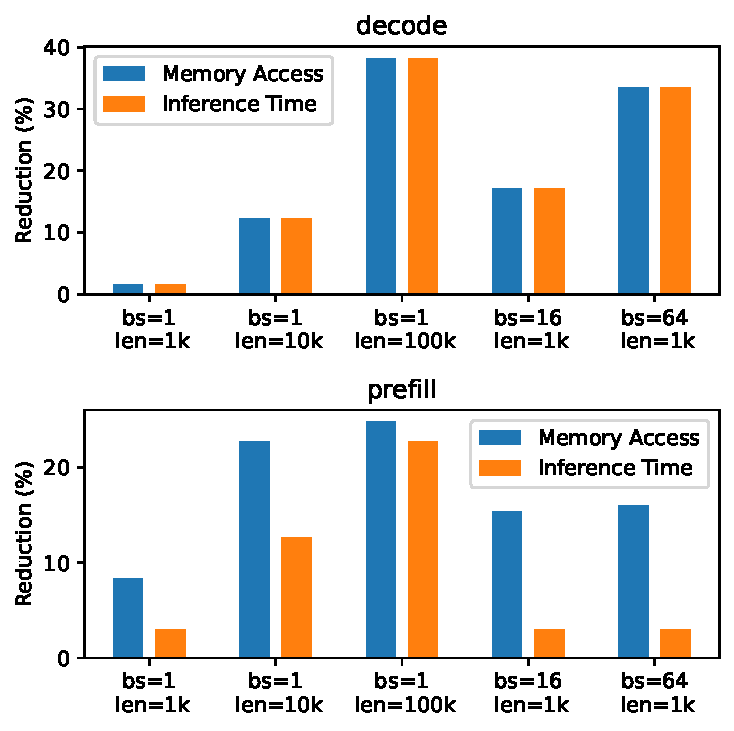
\includegraphics[width=0.95\linewidth]{ims/flashattention_reduction.pdf}
    % \vspace{-0.6in}
    \caption{The memory access reduction and inference time reduction for FlashAttention on Nvidia A6000.}
    \label{fig:flashattention_reduction}
\end{figure}

Operator fusion is an important compile-time optimization technique in deep learning frameworks to improve computational efficiency.
It combines together multiple operators or layers that are directly connected in the computation graph. 
This eliminates redundant data movement and intermediate representations.
For example, a linear operator followed by a SiLU operator can be fused together into a single operator. 
As shown in Figure~\ref{fig:operator_fusion}, this avoids having to store and load the intermediate activations between each operator, reducing both the memory consumption and the memory access.
As shown in Figure~\ref{fig:roofline_operator_fusion}, the roofline model suggests that kernel fusion can increase arithmetic intensity and enhance inference performance in memory-bound areas.
However, when operators are already in a compute-bound area, memory fusion provides little benefit.

While operator fusion can provide significant performance benefits in many cases, it is not applicable to all operators. Operator fusion may not be possible or beneficial for certain operators:
(1) Operator fusion requires that the intermediate results of the fused operations are not needed elsewhere in the computation graph. If a subsequent operation depends on the output of an intermediate operation, fusion is not possible without introducing additional complexity or recomputation.
(2) Operator fusion can potentially increase the on-chip buffer requirements of the fused operation. If the available on-chip buffer is limited, it may not be feasible to fuse certain operations.
(3) Some frameworks or hardware architectures may have limitations or restrictions on which operations can be fused together, depending on their implementation details.

% TODO: 前面challenges部分加一点on-chip buffer的东西

Some compilation tools, such as TVM~\citep{chen2018tvm}, are capable of identifying operators that can be fused together and replacing them with a fused operator. 
However, for LLMs, automatically detecting and fusing operators is both unnecessary and complex because LLMs have a fixed architecture. 
Instead, specific fusion patterns can be used to improve efficiency. 
For instance, the attention mechanism is an essential part of LLMs.
Automatically fusing attention mechanism can be a complex task for compilation tools.
FlashAttention~\citep{dao2022flashattention,dao2023flashattention2} and Flash-Decoding~\citep{dao2023flashdecoding} proposed fusing the matrix multiplications and softmax operator in self-attention into one operator.
This fusion technique eliminates the need to store and load the intermediate attention matrix, which can be very large when the sequence length or batchsize is large. 
As shown in Figure~\ref{fig:flashattention_reduction}, fusing them can significantly decrease the memory access and inference time.
We can observe that there are differences between the prefill stage and decode stage. 
In the decode stage, the memory access reduction is the same as inference time reduction. 
However, in the prefill stage, inference time reduction is lower than memory access reduction. 
This is because some operations in the prefill stage are compute-bound, so reducing memory access by operator fusion provides little benefit.

DeepSpeed-inference~\citep{aminabadi2022deepspeedinference} introduces a technique called Deep-Fusion.
It specifically fuses four main regions within a transformer layer: the QKV GeMM and input layer normalization; transposition and attention operations; post-attention layer normalization and intermediate GeMM; bias addition and residual addition.
xFormers~\citep{xFormers2022} offers various fused kernels that can enhance the performance of transformers. These include fused softmax, fused linear layer, fused layer norm, and fused SwiGLU. 
TensorRT-LLM~\citep{vaidya2023tensorrt_llm} is another framework that offers a wide range of high-performance fused kernels. It incorporates a powerful pattern-matching algorithm that can detect potential fusions in various LLMs. 
% Such operator fusion is widely used in various LLMs inference libraries, such as , vLLM~\citep{kwon2023efficient}, OpenPPL~\citep{sensetime2023openppl}, and TensorRT-LLM~\citep{vaidya2023tensorrt_llm}.

In addition to kernel fusion, we can enhance the performance of the LLM by further optimizing operators' implementation. 
For example, FlashDecoding++~\citep{hong2023flashdecoding++} proposes using asynchronized softmax and flat GEMM optimization with double buffering to improve efficiency.

% through Flash Decoding to search related work

\subsection{Memory Management and Workload Offloading}

When using an LLM to generate responses, the number of input and output tokens can change each time.
The length of the user's input prompt may vary, affecting the length of the sequence in the prefill phase. Additionally, the sequence length increases incrementally during the decode phase as tokens are generated.
This means that the shapes of the activations are not fixed like in a normal neural network. 
How to manage the memory efficiently as the tensor sizes change is a problem. 
PagedAttention~\citep{kwon2023efficient} efficiently handles the KV cache by dividing it into blocks.
The KV cache of each sequence is divided into blocks, with each block containing the keys and values for a fixed number of tokens.
To manage these blocks, a table is used to map the logical blocks of a sequence to the physical blocks in GPU memory.
This mapping is similar to how virtual memory works in a CPU's memory management system.

\begin{figure}[t]
    \centering
    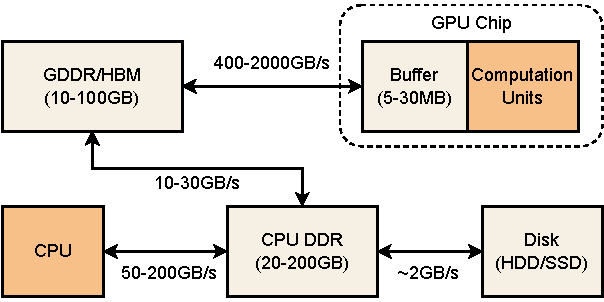
\includegraphics[width=0.9\linewidth]{ims/computer_arch.pdf}
    % \vspace{-0.6in}
    \caption{In typical computer architectures, the memory system consists of different types of memory spaces.}
    \label{fig:computer_arch}
\end{figure}
\begin{figure}[t]
    \centering
    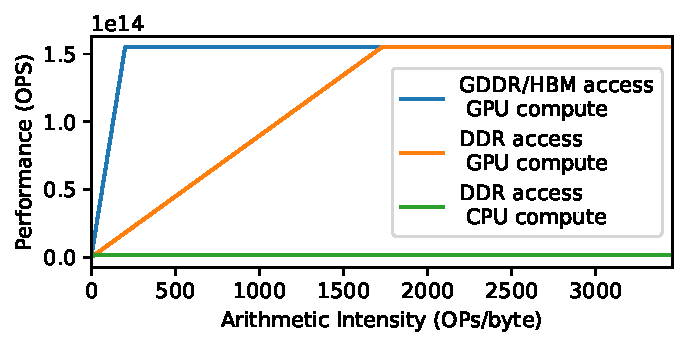
\includegraphics[width=0.9\linewidth]{ims/offloading_roofline.pdf}
    % \vspace{-0.6in}
    \caption{Roofline model for different offload settings.}
    \label{fig:offloading_roofline}
\end{figure}

% However, when the GPU takes a 小memory size，而网络又太大的时候，即使用上了前面所有的方法也无法放下,可以采用workload offloading将网络存储在其它的memory上。
% As shown in Figure~\ref{fig:computer_arch}, 一个计算机系统上有很多不同的memory空间，包括CPU的DDR、GPU的显存、硬盘，但是不同memory的access bandwidth有很大的区别。
% DeepSpeed-inference~\citep{aminabadi2022deepspeedinference} Propose ZeRO-Inference to offload the weights of large models to CPU memory。 This mechanism is able to achieve good performance when using a large batchsize because large batch sizes cause compute time to dominate the latency of fetching model weights, which ultimately improves efficiency.
% 我们还可以利用其它的慢速设备进行计算，例如FlexGen利用CPU进行一部分的计算。

When the GPU has limited memory capacity and the network is too large to fit, it may be necessary to employ workload offloading to store the network in alternative memory spaces.
As depicted in Figure~\ref{fig:computer_arch}, a computer system consists of various memory spaces, including CPU's DDR, GPU's GDDR/HBM, and hard disk. However, these different memory spaces have distinct access bandwidths.
Figure~\ref{fig:offloading_roofline} illustrates that when the data is offloaded to CPU's DDR and transferred to the GPU for computation when needed, it is better than performing the computation on the CPU. When the batch size is large enough, the arithmetic intensity increases significantly, allowing the GPU to fully utilize its computation capacity and achieve good results.
% shows that when the data is offloaded to CPU's  DDR, and transfer them to GPU for compute when needed is better than CPU compute. When the batch size is large enough, leading the arithmetic intensity increase to a large number, it can make full use of the GPU computation capacity and achieve a good result.
DeepSpeed-inference~\citep{aminabadi2022deepspeedinference} introduces ZeRO-Inference, which offloads the weights of large models to CPU memory.
This mechanism performs well with large batch sizes because the increased batch size increase the computation requirement and make the computation latency overlap the latency of fetching model weights, thereby improving overall efficiency.
Huggingface Accelerate~\citep{huggingface2022-accelerate} can also move certain modules to the CPU or disk if there is not enough GPU space to store the entire model.
FlexGen~\citep{sheng2023flexgen} provides a way to explore different ways of offloading computations considering constraints imposed by available hardware resources from the GPU, CPU, and disk. To find the best strategy in terms of throughput, FlexGen employs a linear programming-based search algorithm.
\citet{alizadeh2023llminflash} takes advantage of the larger capacity of flash memory compared to DRAM. It efficiently performs inference by storing model parameters in flash memory and transferring them to DRAM when needed.

\subsection{Parallel Serving}

Parallel serving handles multiple user requests to a server at the same time. One goal is to respond to each request quickly. To achieve this, we need to reduce the time it takes to respond to each user, known as the response latency.
Another important factor to consider is throughput, which is the number of requests the server can process in a given time. By increasing the server's throughput capacity, we can serve more users simultaneously, leading to better overall system performance.
By increasing the server's throughput capacity, more users can be served simultaneously, resulting in improved system performance.
The serving system should be optimized to maximize throughput, while still ensuring that the response latency is within acceptable limits. 
Batching is a fundamental approach to improve throughput by processing multiple user requests together. Figure~\ref{fig:parallel_serving} shows that increasing the batch size during the decode stage significantly enhances throughput. 
However, increasing batch size can increase the response latency and memory consumption.

\begin{figure}[t]
    \centering
    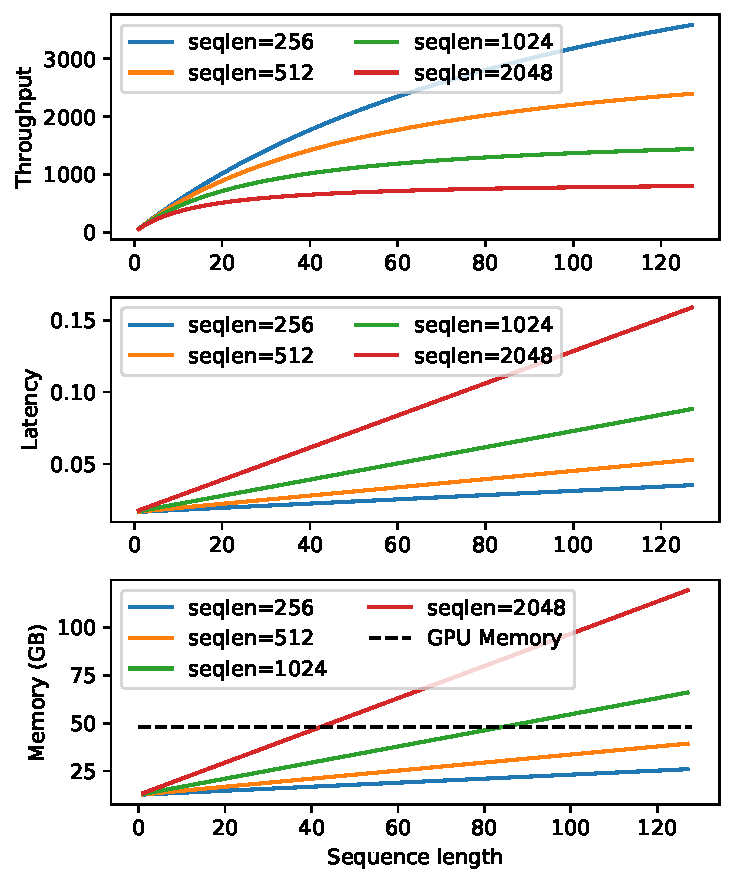
\includegraphics[width=0.9\linewidth]{ims/parallel_serving.pdf}
    % \vspace{-0.6in}
    \caption{The parallel serving settings have an impact on the throughput, latency, and memory usage of the Nvidia A6000 GPU (Llama-2-13b).}
    \label{fig:parallel_serving}
\end{figure}


Several techniques have been proposed to optimize the batching method. For example, ORCA~\citep{yu2022orca} introduces continuous batching (also known as iterative or rolling batching) to combine inferences from different users. 
SARATHI \citep{agrawal2023sarathi} employs chunked-prefills and decode-maximal batching.
It combines prefill chunks and decode requests to create batches, which increases the arithmetic intensity and improves throughput.
Similarly, DeepSpeed-FastGen \citep{holmes2024deepspeedfastgen} and LightLLM \citep{modeltc2024lightllm} also employ a split and fuse technique.

% Batching the inference of different users is one the main methods to improve throughput.
% Figure~\ref{} shows that the performance of decode stage can significantly increased throughput when increasing the batching.
% There are many techniques to optimizing the batching method.
% ORCA~\citep{yu2022orca} propose the continuous batching (also known as iterative or rolling batching) to combine the inference from different users.
% SARATHI~\citep{agrawal2023sarathi}, DeepSpeed-FastGen~\citep{holmes2024deepspeedfastgen}, and LightLLM~\citep{modeltc2024lightllm} use the split the long prompt in prefill stage or combine the inference of decode stage together to get better and more stable inference.

